\documentclass[12pt,a4paper,DIV11]{article}
\usepackage[ngerman]{babel}
\usepackage[utf8]{inputenc} 
\usepackage[T1]{fontenc} 
\usepackage{babel}
\usepackage{ae}
\usepackage{textcomp} 
\usepackage{float}
\usepackage{enumitem}
\usepackage{geometry}
%
\usepackage{fancyref}
\usepackage{fancyhdr} 
\usepackage{amsmath}
\usepackage{xcolor}
\usepackage{url}
\usepackage{makeidx}
\usepackage{listings}
\usepackage{acronym}
%
% PDF settings
\usepackage[pdftex]{graphicx}
\usepackage[pdfstartview=FitH,pdftitle={<Titel>},pdfauthor={<Name>}, colorlinks=false, linktocpage]{hyperref}
\usepackage{svg}
% Header and Footer Style

\geometry{left=35mm, right=25mm, top=25mm, bottom=30mm}

\pagestyle{fancy}
\fancyhead{}
\fancyhead[L]{\slshape\nouppercase{\rightmark}}
\fancyfoot{}
\fancyfoot[C]{\thepage}
\renewcommand{\headrulewidth}{0pt}
\renewcommand{\sectionmark}[1]{\markright{\thesection\ #1}}
\expandafter\def\expandafter\UrlBreaks\expandafter{\UrlBreaks%  save the current one
  \do\a\do\b\do\c\do\d\do\e\do\f\do\g\do\h\do\i\do\j%
  \do\k\do\l\do\m\do\n\do\o\do\p\do\q\do\r\do\s\do\t%
  \do\u\do\v\do\w\do\x\do\y\do\z\do\A\do\B\do\C\do\D%
  \do\E\do\F\do\G\do\H\do\I\do\J\do\K\do\L\do\M\do\N%
  \do\O\do\P\do\Q\do\R\do\S\do\T\do\U\do\V\do\W\do\X%
  \do\Y\do\Z}
%
% No identation
\setlength\headheight{12pt}
\setlength\parindent{0pt} 
%
% Custom commands
\newcommand\zb{z.\,B.\ }
\renewcommand\dh{d.\,h.\ }
\newcommand\parbig{\par\bigskip}
\newcommand\parmed{\par\medskip}
\newcommand{\mailto}[1]{\href{mailto:#1}{#1}}
%
% C# Code Listing Style
\definecolor{darkblue}{rgb}{0,0,.6}
\definecolor{darkgreen}{rgb}{0,0.5,0}
\definecolor{darkred}{rgb}{0.5,0,0}
\lstset{language=[Sharp]C, basicstyle=\ttfamily\small\upshape, commentstyle=\color{darkgreen}\sffamily, keywordstyle=\color{darkblue}\rmfamily\bfseries, breaklines=true,tabsize=2,xleftmargin=3mm, xrightmargin=3mm,numbers=none,frame=single,stringstyle=\color{darkred},
showstringspaces=false}
%
% Titel + Author 
\title{
\includegraphics[width=0.6\textwidth]{pictures/logo}\\
{\normalsize Seminararbeit zum Thema:}\\[6ex]
\huge Sensorlose Indoor-Lokalisierung}
\author{\\Artemij Voskobojnikov, Benjamin Swiers \\
{\normalsize Matrikelnummer: 4557770, ?? }\\
{\normalsize Modul: Seminar Technische Informatik}\\
{\normalsize Dozent: ??}\\
{\normalsize Semester: Sommersemester 2015}\\
}

\date{Berlin, den 17. Juni 2015}



\begin{document}

\begin{titlepage}

\pagenumbering{alph}
\maketitle
\thispagestyle{empty}

\vfill{}

\vfill{}

\end{titlepage}
\clearpage\pagenumbering{Roman}
\include{declaration}
% !TEX encoding = UTF-8 Unicode
\pagestyle{empty}
\section*{Abkürzungsverzeichnis}
\begin{acronym}[Bash]
\acro{AP}{Access Point}
\acro{DfP}{Device-free Passive}
\acro{DfL}{Device-free Localization}
\acro{MP}{Monitoring Point}
\acro{RSSI}{Radio Signal Strength Indication}
\acro{RFID}{Radio Frequency Identication}
\acro{RSSI}{Radio Signalstrength Indication}
\end{acronym}
% !TEX encoding = UTF-8 Unicode
\pagestyle{empty}
\listoffigures
% !TEX encoding = UTF-8 Unicode
\subsection*{Zusammenfassung}
\pagestyle{empty}
In der heutigen Gesellschaft kommen in vielen Bereichen Indoor-Lokalisierungssysteme zum Einsatz. Die Nischen können dabei grundverschieden sein. Neben der Feuerwehr, die Methoden zur Indoor-Lokalisierung verwendet, um Einsatzkräfte oder auch mögliche Opfer in Gebäuden ausfindig zu machen, können Lokalisierungsmethoden auch zur Überwachung von Kindern oder auch älteren Personen verwendet werden.\newline\newline
In dieser Ausarbeitung wird zu Beginn zwischen aktiven und passiven Lokalisierungsmethoden unterschieden und erläutert, was genau passive Lokalisierung ausmacht und welche Vorteile diese gegenüber aktiven Methoden haben. Im weiteren Verlauf werden verschiedene Methoden der passiven Lokalisierung vorgestellt und deren grundlegende Funktionsweise beschrieben. Es werden mögliche Anwendungsgebiete, sowie Vor- und Nachteile der jeweiligen Systeme genannt.\newline\newline Abschließend wird ein Fazit gezogen und auf mögliche Entwicklungen in diesem Forschungsbereich eingegangen. 
\newpage
\pagestyle{empty}
\tableofcontents
\pagestyle{plain}
\clearpage\pagenumbering{arabic}
\setcounter{page}{1}
\include{1_introduction}           
% !TEX encoding = UTF-8 Unicode
\section{Indoor-Lokalisierung}

In dieser Ausarbeitung wird die Indoor-Lokalisierung von Personen betrachtet. Lokalisierung von Objekten ist ebenfalls denkbar, jedoch werden in den heutzutage verwendeten Systeme hauptsächlich Personen lokalisiert. Im Folgenden werden die Begriffe der \textit{aktiven Lokalisierung} und \textit{passiven Lokalisierung} eingeführt und kurz erläutert.

\subsection{Aktive Lokalisierung}
Unter einer \textit{aktiven Lokaliserung} versteht man Lokalisierungsmethoden, welche eine aktive Mitwirkung der Teilnehmer benötigt. Zumeist bedeutet dabei eine aktive Mitwirkung das Tragen eines Gerätes, welches mit den Sensoren im Raum in einer bestimmten Art und Weise kommuniziert.\footnote{Vgl. Deak G.,  Curran K. \& Condell J., S. 1}\\
Solche Systeme sind weit verbreitet, jedoch können Teilnehmer in manchen Situationen keine Gerätschaften bei sich tragen. Ein Beispiel dafür wäre eine Brandsituation. Die Einsatzkräfte der Feuerwehr würden mit aktiven Lokalisierungsmethoden im Regelfall nicht die Opfer ausfindig machen können, was im schlimmsten Fall Menschenleben kosten könnte.\\
Darüber hinaus können Personen selbst kleinste sichtbare Sensoren als unkomfortabel empfinden, sodass in solchen Situationen zu \textit{passiven Lokalisierungsmethoden} gegriffen werden muss.\footnote{Vgl. Kivimäki T., Vuorela T., Peltola P. \& Vanhala J., S.1}
\subsection{Passive Lokalisierung}
Im Gegensatz zur \textit{aktiven Lokalisierungsmethoden} wird bei einer \textit{passiven Lokalisierung} (auch \textit{sensorlose Lokalisierung}) keine aktive Mitwirkung der Teilnehmer verlangt.\footnote{Vgl. ebd.} Ein großer Vorteil solcher Systeme ist die Benutzerfreundlichkeit, da keinerlei Gerätschaften sich am Teilnehmer selbst befinden müssen. Ebenfalls bieten \textit{sensorlose Lokaliserungsmethoden} neue Anwendungsbereiche wie zum Beispiel Alarmanlagen in Gebäuden. So können Einbrecher lokalisiert werden, was bei \textit{aktiver Lokalisierung} nur schwer vorstellbar ist.\\
Die folgende Abbildung zeigt nochmals die Unterkategorien von \textit{Indoor-Lokalisierung} auf:

\begin{figure}[H]
	\centering
	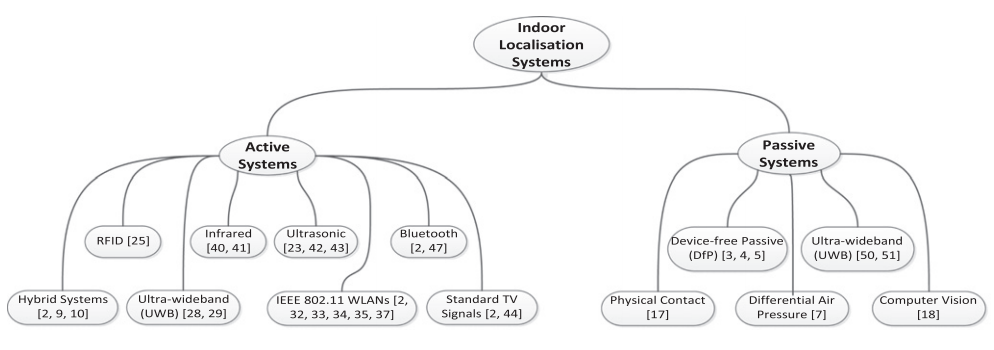
\includegraphics[scale=0.9]{pictures/indoor_loc}
	\caption{Unterkategorien von Indoor-Lokalisierung (Deak G.,  Curran K. \& Condell J., S. 2)}
\end{figure}

Im weiteren Verlauf wird jedes \textit{passive System} näher untersucht. Es wird die Funktionsweise sowie die Vor- und Nachteile des jeweiligen Systems erläutert.


\section{Sensorlose Indoor-Lokalisierung}
\subsection{Radio Frequency Identification}
Unter \textit{Radio Frequence Identification} (\textbf{RFID}) versteht man eine kontaktlose Identifikation mittels Funkübertragung. Oftmals kann man hierfür bereits vorhandene Wi-Fi-Netzwerke verwenden.\footnote{Vgl. Kivimäki T., Vuorela T., Peltola P. \& Vanhala J., S.  16} \\
Ein solches DfL-System (\textbf{Device-free Localization}) nutzt die Tatsache aus, dass die Präsenz eines menschlichen Körpers die Radiosignale beeinflusst.\footnote{Vgl. ebd.} Die verwendete Frequenz der Knotenpunkte liegt hierbei bei $2.4$Ghz, weil dies die Resonanzfrequenz von Wasser ist und der Mensch bekanntermaßen aus $70\%$ aus Wasser besteht.\footnote{Vgl. Deak G.,  Curran K. \& Condell J., S. 11}. Ein weiterer Pluspunkt ist auch, dass die Frequenz von $2.4$ Ghz bei \textit{IEEE Standards} wie $802.11b$ und $802.11g$ verwendet wird.\footnote{Vgl. Pirzada N.,Nayan Y., Subhan F., Hassan F., Khan M., S. 3}\\
Das \textit{DfP-System} (\textit{Device-free Passive}) auf Grundlage von \textit{RFID}, welches im Folgenden vorgestellt wird, misst die Änderungen von der erhaltenen \textit{Received Signal Strength Indication} (\textbf{RSSI}). Systeme, die von der \textit{RSSI} Gebrauch machen, haben meist eine Genauigkeit von bis zu $18$cm.\footnote{Vgl. Deak G.,  Curran K. \& Condell J., S. 14}. Das in folgendenen Abschnitten vorgestellte System soll als Alarmanlage agieren und Eindringlinge lokalisieren bzw. detektieren können.\footnote{Vgl. Mah M., S. 2} Ein solches System besteht aus zwei Komponenten, den \textit{Access Points} (\textbf{AP})\footnote{Z. Dt. Zugriffsknoten} und den \textit{Monitoring Points} (\textbf{MP})\footnote{(Z. Dt. Kontrollknoten)}. Einen guten Überblick bietet die folgende Abbildung:\\

\begin{figure}[H]
	\centering
	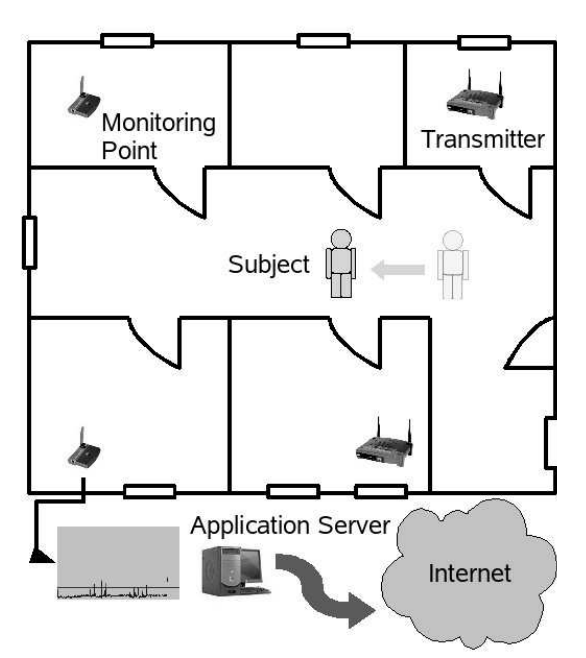
\includegraphics[width=0.5\textwidth]{pictures/rfid}
	\caption{RFID Indoor-Lokalisierung (Mah M., S. 2)}
\end{figure}

In der obigen Abbildung erkennt man zwei \textbf{AP}, sowie einen \textbf{MP} und einen \textbf{DfP Server}, der die Berechnungen auf Grundlage der erhaltenen Signale durchführt. Als \textbf{MP} können dabei beliebige Computer verwendet werden.\footnote{Vgl. ebd.} Neben der eigentlichen Detektion (\textit{Monitoring Mode}) unterstützt das System noch zwei weitere Modi, welche nun näher beschrieben werden.\\

\begin{itemize}
\item \textbf{Monitoring Mode}: Dieser Modus nimmt jegliche Aktivität wahr, eignet sich somit für eine nächtliche Überwachung.
\item \textbf{Tracking mode}: Dieser Modus kann einen Eindringling orten und zusätzlich noch anhand der Daten der, die von den \textbf{MP} verzeichnet werden, verfolgen. Es kann nur ein Eindringling zu einem bestimmten Zeitpunkt geortet werden.
\item \textbf{DfP Mode}: Der \textit{DfP-Modus} kann mehrere Eindringlinge gleichzeitig orten und verfolgen.
\end{itemize}

Sobald ein Eindringling von einem \textbf{MP} detektiert wird, werden zusätzlich noch weitere \textit{Monitoring Points} kontaktiert und auf mögliche Detektionen überprüft. Erst danach kommt es zu einem Alarm des Gesamtsystems.\footnote{Vgl. ebd., S. 2 f.} Der zentrale Alarm kann hierbei auf disjunkten Paaren von \textbf{AP} und \textbf{MP} basieren. Aus diesem Grund ist es notwendig die Detektionen möglichst simultan zu verzeichnen.\footnote{Vgl. ebd.}

\subsection{Experimenteller Aufbau}
Es wurden vier Experimente in kontrollierter Umgebung durchgeführt. Die eigentliche Leistung des Systems konnte somit besser untersucht werden, da die äußeren Einflüsse dadurch minimiert wurden. Bei jedem einzelnen Experiment wurde eine bestimmte Anordnung von zwei \textbf{AP} und zwei \textbf{MP} verwendet. Jeder \textbf{MP} zeichnete dabei die \textit{RSSI} von jedem \textbf{AP} auf, die alle $100$ ms sendeten.\\
Ein beispielhafter Aufbau ist in der folgenden Abbildung (links) zu sehen:

\begin{figure}[H]
\centering
\begin{minipage}{.5\textwidth}
  \centering
	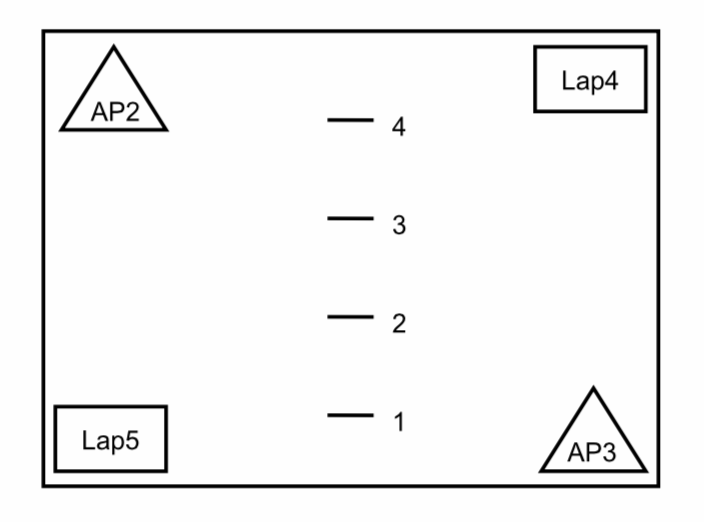
\includegraphics[scale=0.6]{pictures/experiment}
	\caption*{Aufbau}
\end{minipage}%
\begin{minipage}{.5\textwidth}
  \centering
  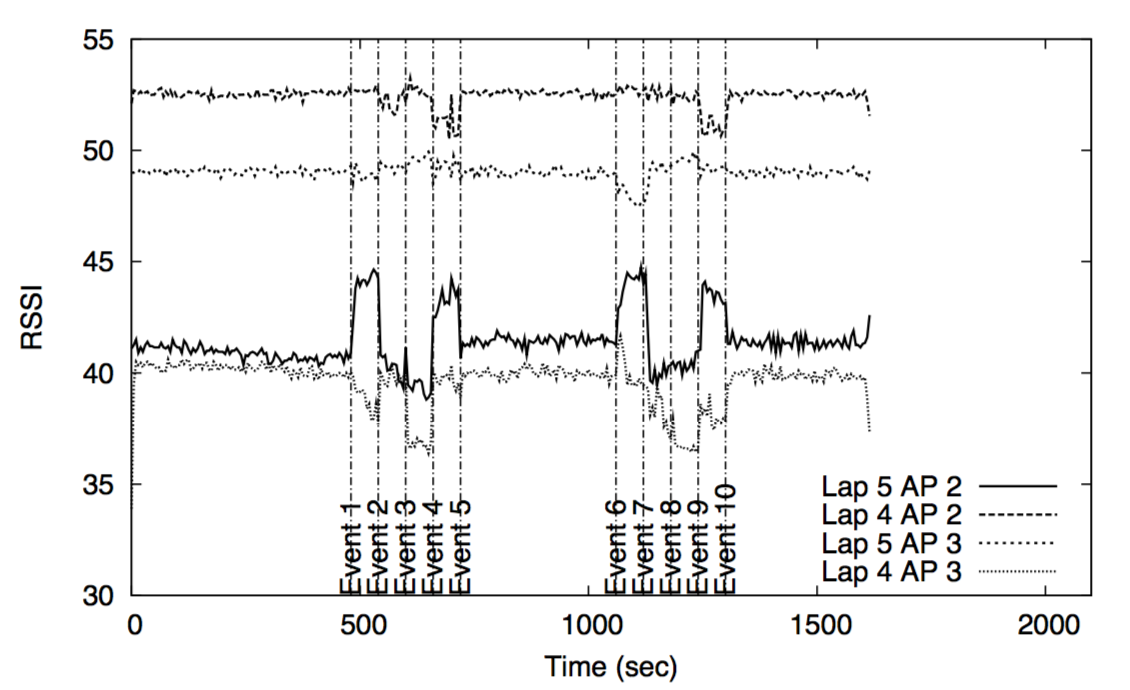
\includegraphics[scale=0.45]{pictures/versuch}
  \caption*{Versuchsverlauf}
\end{minipage}
\caption{Eines der vier Experimente (Mah M., S. 4)}
\end{figure}

Jeder \textbf{MP} zeichnete dabei 1800 Sekunden auf. Eine Person durchlief während dieses Zeitraumes den Raum und hielt an vier Positionen für jeweils 60 Sekunden an. Nach Durchqueren verließ die Person den Raum und das Experiment wurde danach wiederholt. Diese vier Positionen sind in der obigen linken Abbildung mittig zu sehen. Auf der rechten Abbildung sind die Detektionen der jeweiligen \textbf{AP} dargestellt. Dabei wurden alle möglichen Paare von \textbf{AP} und \textbf{MP} untersucht.

\subsection{Testergebnisse}
 Tests in kontrollierten Umgebungen ergaben zufriedenstellende Ergebnisse mit einer niedrigen Rate von \textit{False Positives}\footnote{Z. Dt. Falschpositiv} und einer hohen \textit{Detektionsrate}. Hierbei bedeuten \textit{False Positives} die Detektionen, die fälschlicherweise enstanden sind, es also eigentlich keinerlei Bewegung zu verzeichnen gab. Die \textit{Detektionsrate} gibt die relative Häufigkeit von korrekten Detektionen an. Die beiden beiden folgenden Abbildungen zeigen dies nochmals graphisch auf.

\begin{figure}[H]
\centering
\begin{minipage}{.5\textwidth}
  \centering
  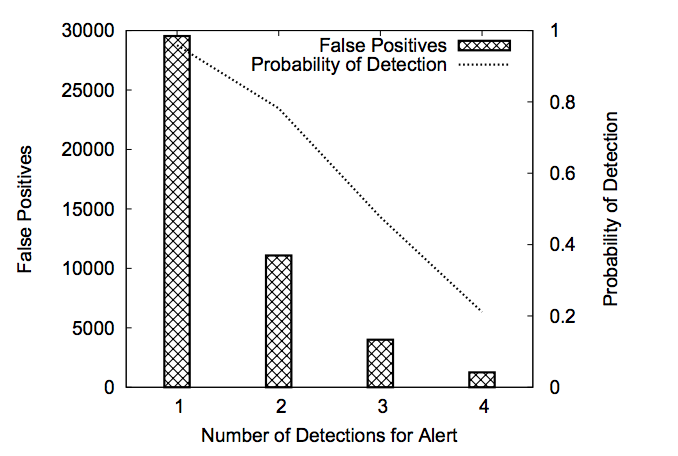
\includegraphics[scale=0.6]{pictures/false_pos}
  \caption*{False Positives}
\end{minipage}%
\begin{minipage}{.5\textwidth}
  \centering
  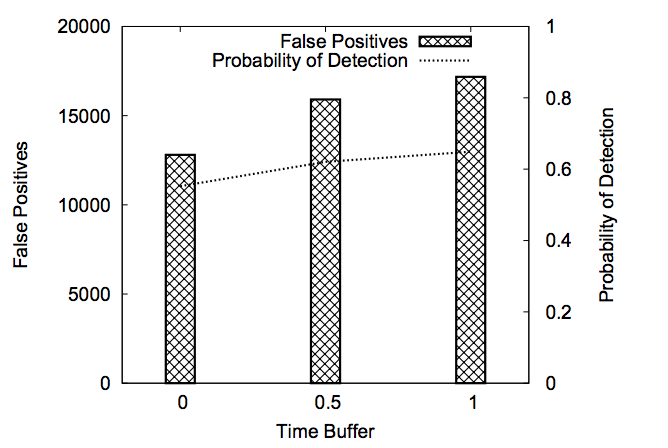
\includegraphics[scale=0.6]{pictures/detection}
  \caption*{Detection Rate}
\end{minipage}
\caption{Testergebnisse (Mah M., S. 9)}
\end{figure}

Dieses \textit{DfP-System} schnitt in den Tests zufriedenstellend ab, jedoch muss man auch auf mögliche Schwachstellen eingehen. Viele Parameter, die in den Algorithmen\footnote{Moving Variance Based Detection \& Moving Average Based Detectionn \url{https://www.cs.umd.edu/sites/default/files/scholarly_papers/MatthewMah_1.pdf}} für die Detektion von Eindringlingen gebraucht werden haben direkten Einfluss auf die Sensibilität des Systems. Will man die Wahrscheinlichkeit eine korrekte Detektion zu verzeichnen erhöhen, wird gleichzeitig die Anzahl der \textit{False Positives} erhöht, die beiden Größen stehen also in direkter Korrelation zueinander. Das Finden von Parametern, welche die Wahrscheinlichkeit von Detektionen erhöhen und gleichzeitig die Anzahl der \textit{False Positives} minimieren, ist ein Optimierungsproblem.\footnote{Vgl. ebd. S. 9}

\subsection{Ultra-wideband}

\textit{Ultra-wideband}\footnote{Z. Dt. Ultrabreitband} (\textbf{UWB}) ist eine weitere Methode Objekte zu lokalisieren. Bei \textbf{UWB} werden sehr große Frequenzbereiche zur Nahbereichskommunikation verwendet. Dabei werden vier Arten von UWB-Imaging\footnote{Z. Dt. Darstellung} unterschieden:\footnote{Vgl. Deak G.,  Curran K. \& Condell J., S. 12}
\begin{itemize}
 	\item \textbf{Ground Penetrating Radar}: Detektion vergrabener Objekte 
 	\item \textbf{Wall Imaging}: Detektion von Objekten innerhalb dichter Wände
 	\item \textbf{Through-wall Imaging}: Detektion von Objekten oder Personen auf der anderen Seite einer Wand
 	\item \textbf{Medical Imaging}: Verwendung für medizinische Zwecke
 \end{itemize} 

Das erste System, was eine Überwachung durch Wände ermöglichte, verwendete Signale mit einer Frequenz zwischen $902$ und $928$ MHz. Dieses System war in der Lage sich bewegende Objekte mit bis zu $1.5$ $m/s$ zu detektieren. Wurde eine Bewegung detektiert, so wurde vom Empfänger ein akkustisches Signal ausgelöst. Der Nachteil dieses Systems war jedoch, dass das Signal Wände mit Spiegeln oder allgemein nasse Wände nur schlecht penetrieren konnte. Systeme, die hingegen auf \textbf{UWB} basieren, verwenden Frequenzen von $3.1$ bis $10.6$ GHz, die eine Penetration von Wänden ermöglichen. Darüber hinaus sind diese Systeme resistenter gegenüber Interferenz sowie Multipath-Fading,\footnote{Z. Dt. Mehrwegempfang}\footnote{Vgl. ebd.} also gegenüber einem Empfang eines gleichen Signals auf unterschiedlichen Wegen. Dies kann beispielsweise aufgrund von Brechung oder Reflektion entstehen, wie die untere Abbildung zeigt.\\

\begin{figure}[H]
	\centering
	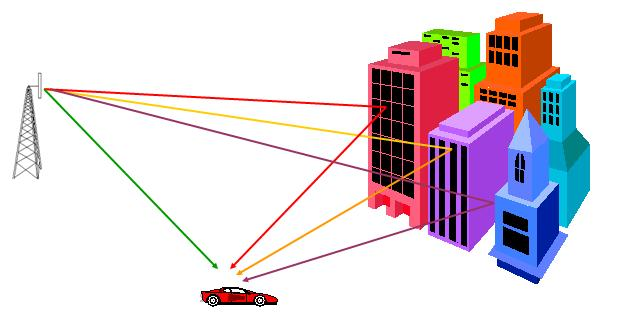
\includegraphics[width=0.6\textwidth]{pictures/multi}
	\caption{Multipath-Fading (Teletopix)}
\end{figure}

\textbf{UWB}-Systeme beheben viele der Probleme, die bei \textit{Narrowband}-Systemen\footnote{Z. Dt. Schmalband} entstehen können, gleichzeitig gibt es, wie bei jedem System, aber auch Kehrseiten. Zwar wurden Experimente mit \textbf{UWB}-Lokalisierungssystemen durchgeführt, es gibt jedoch keine einheitlichen Methoden zur Detektion von Objekten und zur Verarbeitung der Signale. Ebenso muss in der Mehrheit der existierenden Systeme eine Lerndatenbank gepflegt werden, die erstellt werden muss bevor die eigentliche Lokalisierung vonstattengehen kann.\footnote{Vgl. Kilic Y., Wymeersch H., Meijerink A., Bentum M. \& Scanlon W., S. 1}\\
Abschließend kann man sagen, dass Systeme, die auf Radiosignalen basieren ihren Zweck erfüllen, es jedoch kein universelles System gibt und man je nach Einsatzgebiet ein passendes Verfahren auszuwählen hat.


\subsection{Passive Infrarot-Lokalisierung}
Die passive Infrarot-Lokalisierung (\textbf{PIL}) basiert auf der Körperwärmestrahlung einer Person bzw. eines Objektes. Der thermische Unterschied eines Objektes im Vergleich zu seiner Umgebung kann dabei zur Lokalisierung und Bewegungsverfolgung (Tracking) ausgenutzt werden. Die untere Abbildung zeigt die unterschiedliche Wärmestrahlung einer Person und gegenüber seiner Umgebung.

\begin{figure}[H]
	\centering
	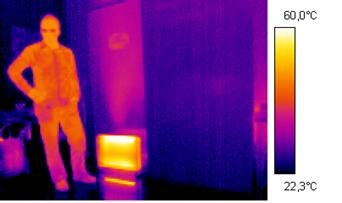
\includegraphics[width=0.5\textwidth]{pictures/pil1}
	\caption{Wärmestrahlung einer Person (Technische Universität Dortmund (2015))}
\end{figure}

Die Detektion der Wärmestrahlung wird durch sogenannte Thermopiles\footnote{Z. Dt. Thermosäulen}  realisiert.\footnote{Vgl. Technische Universität Dortmund 2015} Dabei handelt es sich um elektronische Bauelemente, welche thermische Energie in elektrische Energie umwandeln.\footnote{Vgl. Kemper 2010, S. 33} Um eine Person zu lokalisieren bzw. zu tracken, werden mehrere dieser Sensoren im Raum positioniert, um die thermischen Unterschiede zu messen. Auf Grundlage der so ermittelten Daten können anschließend mit Hilfe spezieller Algorithmen die Sichtwinkel auf die entsprechende Person berechnet werden. Durch Triangulation kann durch diese Winkel die Position eines Objektes bestimmt werden.\footnote{Vgl. Technische Universität Dortmund 2015} Die untere Abbildung skizziert dieses Verfahren.

\begin{figure}[H]
	\centering
	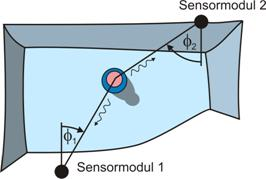
\includegraphics[width=0.5\textwidth]{pictures/triangulation}
	\caption{Lokalisierung durch Triangulation (Technische Universität Dortmund (2015))}
\end{figure}

Der Vorteil dieser Methode liegt nicht nur in der Tatsache, dass ein zu lokalisierendes Objekt keine zusätzliche Hardware mitführen muss. Durch den Verzicht bildgebender Sensoren wird zusätzlich ein Schutz der Privatsphäre gewährleistet.\footnote{Vgl. Kemper 2010, S. 149} Weiterhin ist diese Art der Lokalisierung gegenüber anderen Methoden vergleichsweise kostengünstig.\footnote{Vgl. Kemper 2010, S. 149}\footnote{Vgl. Deak G., Curran K. \& Condell J., S. 7}Da sich die Kosten für Bauteile und Sensoren rasant verändern, ist diese Aussage keinesfalls allgemeingültig. 

\subsection{Differential Air Pressure}
Eine weitere Möglichkeit der Lokalisierung bietet die Messung der Luftdruckschwankungen, die durch ein sich bewegendes Objekt ausgelöst werden. Wenn eine Person eine Tür öffnet, hat dies eine, durch entsprechende Sensoren messbare, kurzzeitige Veränderung des Luftdrucks innerhalb eines Systems zur Folge.\footnote{Vgl. Deak G., Curran K. \& Condell J., S. 13} Dieser Effekt tritt, in abgeschwächter Form, auch beim Passieren eines Engpasses, z.B. eines Türrahmens, auf. Die folgende Abbildung zeigt die Veränderung der Messwerte beim Öffnen/Schließen einer Tür (links) und beim Durchschreiten des Türrahmens (rechts).

\begin{figure}[H]
	\centering
	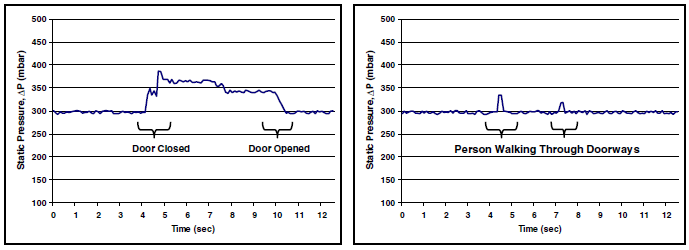
\includegraphics[width=1.0\textwidth]{pictures/dap_diagramm}
	\caption{Detektion von Bewegungen durch Luftdruckänderungen( Patel Shwetak N., Reynolds Matthew S., Abowd Gregory D., S. 7)}
\end{figure} 

Im Gegensatz zu vielen anderen Lokalisierungsmethoden müssen die Sensoren zur Datenerfassung nicht an vielen Stellen des Raumes angebracht werden. Die meisten modernen Häuser verfügen über eine Klimaanlage, welche die Bewohner des Hauses einerseits mit Frischluft versorgt und andererseits die verbrauchte Luft aus dem Haus leitet.\footnote{Patel Shwetak N., Reynolds Matthew S., Abowd Gregory D., S. 2} Dieses Lüftungssystem wird bei der Differential Air Pressure-Methode genutzt, um die Veränderungen des Luftdrucks an einer zentralen Stelle zu erfassen. In der folgenden Abbildung ist ein Klimaanlagensystem eines Hauses abgebildet. 

\begin{figure}[H]
	\centering
	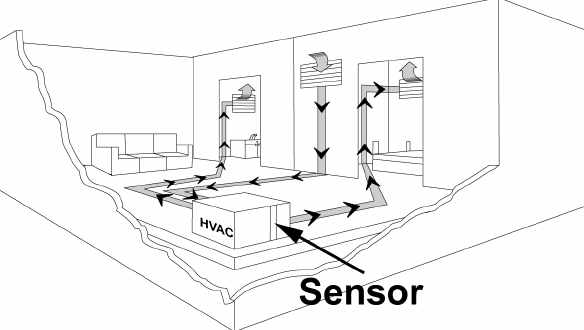
\includegraphics[width=0.6\textwidth]{pictures/dap_klima}
	\caption{Detektion von Bewegungen durch Luftdruckänderungen( Patel Shwetak N., Reynolds Matthew S., Abowd Gregory D., S. 7)}
\end{figure} 

Da die Sensoren in der zentralen Stelle angebracht werden können, kann auf die Installation zusätzlicher Hardware innerhalb des Wohnbereichs verzichtet werden. Der Nachteil diese Methoden liegt in der relativ geringen Genauigkeit bei der Positionsbestimmung. Man kann zwar sagen, in welchem Raum sich eine Person befindet, nicht jedoch an welcher Stelle des Raumes.

\subsection{Physical Contact}
Eine vergleichsweise unauffällige Methode zur Lokalisierung bilden Verfahren, die auf dem physischen Kontakt einer Person zu seiner Umgebung bzw. zu seinem Untergrund beruhen. \footnote{Vgl. Deak G., Curran K. \& Condell J., S. 12} Bei den meisten Verfahren, die auf dem physischen Kontakt basieren, werden sogenannte Piezoelemente zur Detektion eingesetzt. Bei Piezoelementen handelt es sich um ein elektrisches Bauteil, welches die elektrische Polarisation und somit auftretende elektrische Spannung an einem Festkörper messen kann, welche auftritt, wenn das Bauteil elastisch verformt wird. \footnote{Vgl. Peelamedu, Saravanan M., S. 2093} \newline\newline
Diese Piezoelemente werden häufig in Form von Matten in den Boden integriert. Da sich diese unter gebräuchlichen Bodenbelägen, wie Teppichen o.Ä., verlegen lassen, kann dieses System sehr unauffällig in die Umgebung des Hauses integriert werden. Die Möglichkeiten, die dieses System bietet, geht weit über die reine Lokalisierung und Bewegungserkennung hinaus.
Abhängig von der Anzahl der verwendeten Piezoelemente bzw. deren Abstand zueinander, kann ein recht hoher Genauigkeitsgrad erreicht werden, der es erlaubt bestimmte Druckmuster zu erkennen, durch die nicht nur die Position einer Person ermittelt werden kann, sondern darüber hinaus auch die Haltung dieser Person. Die untere Abbildung zeigt ein Druckmuster, wie es bei einem Sturz einer Personen entstehen kann.\\

\begin{figure}[H]
	\centering
	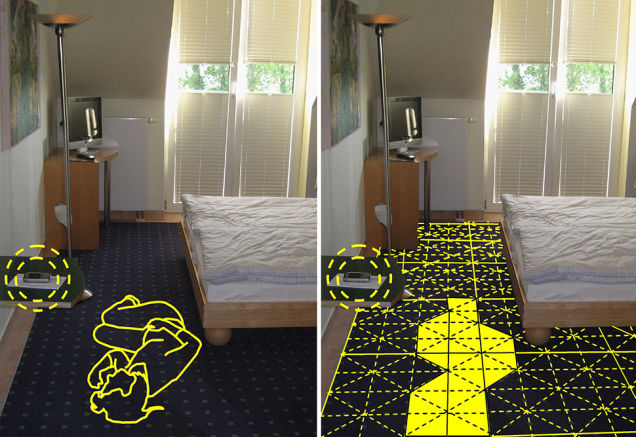
\includegraphics[width=0.6\textwidth]{pictures/piezo}
	\caption{Detektionen eines Sturzes( \url{http://i.kinja-img.com/gawker-media/image/upload/s--WB7wQYq6--/c_fit,fl_progressive,q_80,w_636/19gzk7od0artwjpg.jpg})}
\end{figure} 

Sollte ein Sturz erkannt werden, so könnte automatisch ein Notruf abgesetzt werden, durch den Hilfe angefordert wird. Diese Funktionalität könnte in Haushalten eingesetzt werden, in denen alte oder körperlich beeinträchtigte Personen leben.\newline\newline
Eine weitere Möglichkeit den physischen Kontakt ein Person zu zur Lokalisierung zu Nutzen, ist die Tatsache, dass ein eine Person bei dem Kontakt mit dem Untergrund einen Abdruck erzeugt.
 
\subsubsection{Projekt: GravitySpace}
Am Hasso-Plattner-Institut in Potsdam wurde ein Verfahren entwickelt, welches sich diesen Effekt zu Nutze macht. 
Für den Versuchsaufbau dieses Verfahrens wurde als Bodenplatte eines Zimmers eine Glasscheibe verwendet, welche von unter mit einer Kamera gefilmt wird. Die Abbildung ... zeigt diesen Versuchsaufbau.

\begin{figure}[H]
	\centering
	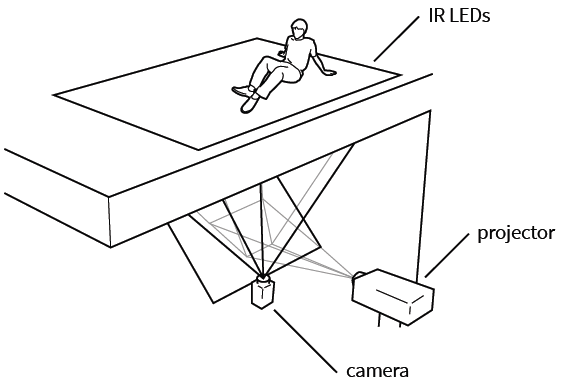
\includegraphics[width=0.6\textwidth]{pictures/hpi1}
	\caption{Versuchsaufbau GravitySpace(Bränzel et al., S. 2)}
\end{figure}

Bränzel et al.

\subsection{Computer-Vision}
Auch Computer-Vision kann als \textbf{DfP}-System betrachtet werden, da ein potentieller Nutzer keine zusätzliche Hardware am Körper tragen muss. Das Ziel dieses Systems ist, eine Umgebung zu schaffen, die auf die Position und das Verhalten einer Person reagiert (intelligente Umgebung). \footnote{Vgl. Deak G., Curran K. \& Condell J., S. 13}\newline Es ist beispielsweise vorstellbar, dass 

Test

\subsection{Fazit und Ausblick}
In dieser Ausarbeitung wurden verschiedene Methoden zur Lokalisierung und Bewegungsverfolgung von Person innerhalb von Gebäuden vorgestellt. Dabei wurden die Funktionsweisen der jeweiligen Methoden erläutert und deren Vor- und Nachteile aufgezeigt.\newline\newline 
Zusammenfassend lässt sich sagen, dass jede Methode seinen Einsatzzweck hat und der Vergleich der Technologien untereinander nur bedingt sinnvoll ist. Abhängig vom Einsatzzweck liegt das Augenmerk auf unterschiedlichen Eigenschaften und Anforderungen. Nicht jede Methode kann den entsprechenden Anforderungen gerecht werden. Obwohl die vorgestellten Systeme im Grunde die gleiche Aufgabe erfüllen, so unterscheiden sie sich doch in vielerlei Punkten. Die Genauigkeit, der Installationsaufwand und letztlich auch der Preis stellen hier nur einige dieser Punkte dar. \newline\newline
Im Laufe der Zeit werden die Bauteile für solche Systeme voraussichtlich immer günstiger, wodurch der finanzielle Aspekt zunehmend vernachlässigbar werden wird. Der technologische Fortschritt wird weiterhin präzisere und kleine Sensoren mit sich bringen, wodurch eine Bewertung der verschiedenen Systeme in einigen Jahren deutlich andere Ergebnisse liefern würde. 

\newpage

\section{Quellenverzeichnis}
\subsection*{Literaturquellen}
\begin{itemize}[leftmargin=*]
\item[] \textbf{Sample}
\end{itemize}
\subsection*{Sonstige Quellen}
\begin{itemize}[leftmargin=*]
\item[] \textbf{Bränzel et al.}: GravitySpace: Tracking Users and Their Poses in a Smart Room Using a Pressure-Sensing Floor (2013), Online unter URL: \url{https://hpi.de/fileadmin/user_upload/fachgebiete/baudisch/publications/GravitySpace_CHI2013.pdf}
\item[] \textbf{Deak G., Curran K. \& Condell J.} A survey of active and passive indoor localisation systems (2012), Online unter URL : \url{http://scisweb.ulster.ac.uk/~kevin/comcomsurvey.pdf}
\item[] \textbf{Ehrlich, I.}: Indoor Localization (2006), Online unter URL: \url{http://ifgi.uni-muenster.de/~muellerj/lbs06/proceedings/3-IndoorLocalization.pdf}
\item[] \textbf{Kemper J.}: Passive Infrarot-Lokalisierung (2010), Fakultät für Elektrotechnik und Informationstechnik, Technischen Universität Dortmund, Dortmund, Online unter URL: \url{https://eldorado.tu-dortmund.de/bitstream/2003/27428/1/PIL.pdf}
\item[] \textbf{Kilic Y., Wymeersch H., Meijerink A., Bentum M. \& Scanlon W.}: Online unter URL: \url{http://arxiv.org/pdf/1303.4092.pdf}
\item[] \textbf{Kivimäki T., Vuorela T., Peltola P. \& Vanhala J.}: A Review on Device-Free Passive Indoor Positioning Methods (2014), Online unter URL: \url{http://www.sersc.org/journals/IJSH/vol8_no1_2014/9.pdf}
\item[] \textbf{M. Mah}: Device-Free Passive Localization (2007), Online unter URL: \url{https://www.cs.umd.edu/sites/default/files/scholarly_papers/MatthewMah_1.pdf}
\item[] \textbf{Pirzada N., Nayan Y., Subhan F., Hassan F., Khan M.}: Device-Free Localization Technique for Indoor Detection and Tracking of Human Body (2013), Online unter URL: \url{http://ac.els-cdn.com/S187704281402878X/1-s2.0-S187704281402878X-main.pdf?_tid=7bc6ad0e-12a4-11e5-95f4-00000aab0f02&acdnat=1434293516_4a2274a0ebfb932cf57c3f4f652c668f}
\item[] \textbf{Patel Shwetak N., Reynolds Matthew S., Abowd Gregory D.}: Detecting Human Movement by Differential Air
Pressure Sensing in HVAC System Ductwork: An Exploration in Infrastructure Mediated Sensing (2008), College of Computing, School of Interactive Computing, \& GVU Center Georgia Institute of Technology, Online unter URL: 
\url{https://dub.washington.edu/djangosite/media/papers/tmpqiqC-3.pdf}
\item[] \textbf{Peelamedu, Saravanan M.}: Piezoelectric Effect and Its Application, in Encyclopedia of Optical Engineering, hrsg. v. Ronald G. Driggers, 2003
\item[] \textbf{Technische Universität Dortmund}: TU Dortmund, Fakultät ETIT, IRF, IT, Forschung, Embedded Systems,  Projekte, PIL, DFG-Projekt: Passive Infrarot-Lokalisierung, Online unter URL: \url{http://www.irf.tu-dortmund.de/cms/de/IT/Forschung/Embedded_Systems/Projekte/PIL/index.html}, Abruf: 2015-06-15
\item[] \textbf{Teletopix: Multipath-Fading}: Online unter URL: \url{http://www.teletopix.org/wp-content/uploads/2013/01/MUltipath-effect.jpg}, Abruf: 2015-06-26
\end{itemize}


\bibliographystyle{alpha}

\end{document}
